\documentclass{article}

% NeurIPS style
\usepackage[final]{neurips_2024}

\usepackage[utf8]{inputenc}
\usepackage[T1]{fontenc}
\usepackage{hyperref}
\usepackage{url}
\usepackage{booktabs}
\usepackage{amsfonts}
\usepackage{amsmath}
\usepackage{nicefrac}
\usepackage{microtype}
\usepackage{xcolor}
\usepackage{graphicx}
\usepackage{subcaption}

\title{Desire-Likeness is Multi-Dimensional: Comparing Behavioral Signatures Across Learning Frameworks}

\author{%
  Paul Fryer
}

\date{January 27, 2026}

\begin{document}

\maketitle

\begin{abstract}
We investigate whether Active Inference agents exhibit behavioral signatures distinguishing them from Reinforcement Learning agents. Using a grid-world foraging task, we compare five agent types---heuristic, PPO, DQN, A2C, and Active Inference---across six behavioral predicates drawn from the psychology of motivation. Contrary to initial hypotheses, we find no clean dissociation between frameworks. Instead, we discover that ``desire-likeness'' is multi-dimensional: Active Inference and value-based RL (DQN) both show \textit{true anticipatory activation} ($r \approx -0.6$), while actor-critic methods (A2C) show the strongest state-dependent valuation and frustration response. Notably, PPO shows \textit{inverse anticipation}---activation that increases with distance from goals ($r = +0.63$), encoding uncertainty rather than goal proximity. These results suggest that the architecture of learning systems, not merely the framework (RL vs.\ Active Inference), determines which aspects of goal-directed behavior emerge. We propose that future work should measure multiple ``desire signatures'' rather than seeking single dissociating predicates.
\end{abstract}

\section{Introduction}

The question of whether artificial agents can possess states analogous to desires, goals, or intentions has both practical and philosophical significance \cite{dennett1987intentional, bratman1987intention}. In practical terms, understanding the internal dynamics of agents may help predict their behavior in novel situations. Philosophically, it touches on debates about the nature of agency and whether goal-directedness is merely a useful description or reflects genuine internal structure.

Active Inference \cite{friston2010free, parr2022active} offers an alternative to standard reinforcement learning that is explicitly framed in terms of beliefs and preferences rather than rewards. Agents minimize \textit{expected free energy}, which combines epistemic value (information gain) with pragmatic value (achieving preferred states). This formulation naturally incorporates prospective planning and has been argued to produce more ``desire-like'' behavior \cite{seth2021being}.

However, behavioral equivalence poses a challenge: any behavior produced by one agent class can often be reproduced by another with appropriate reward shaping or architecture. To distinguish agents meaningfully, we need \textit{behavioral predicates}---specific patterns that may dissociate agent types even when overall task performance is similar.

Drawing on the psychological literature on motivation and desire \cite{berridge2009dissecting}, we propose six behavioral predicates:
\begin{enumerate}
    \item \textbf{Anticipatory Activation (AA)}: Correlation between internal state activity and proximity to goals
    \item \textbf{Frustration Intensification (FI)}: Activity spike when expected paths are blocked
    \item \textbf{Opportunity Cost Sensitivity (OCS)}: Rational weighing of alternatives
    \item \textbf{Extinction Resistance (ER)}: Persistence of behavior when rewards cease
    \item \textbf{State-Dependent Valuation (SDV)}: Valuation that varies with internal state (e.g., energy level)
    \item \textbf{Means-End Decoupling (MED)}: Flexibility in transferring to new paths
\end{enumerate}

Our initial hypothesis was that Active Inference would uniquely exhibit anticipatory activation due to its explicit prospective planning. However, our results reveal a more nuanced picture: desire-likeness is multi-dimensional, and different agent architectures exhibit different ``desire signatures.''

\section{Related Work}

\paragraph{Active Inference and Agency.} Active Inference \cite{friston2010free} frames perception and action as inference under a generative model. Agents select actions to minimize expected free energy, balancing exploration (reducing uncertainty) with exploitation (achieving preferred states). This framework has been applied to robotics \cite{lanillos2021active}, neuroscience \cite{parr2022active}, and cognitive modeling \cite{smith2022step}.

\paragraph{Behavioral Signatures of Goal-Directedness.} The distinction between goal-directed and habitual behavior has a long history in psychology \cite{dickinson1985actions}. Goal-directed behavior is sensitive to outcome devaluation and contingency degradation, while habitual behavior persists regardless. Recent work has begun applying these concepts to artificial agents \cite{langdon2022model}.

\paragraph{Comparing RL and Active Inference.} Several studies have compared RL and Active Inference agents on specific tasks \cite{millidge2020relationship, tschantz2020reinforcement}. Most find behavioral equivalence under appropriate conditions. Our contribution is to show that single predicates can mislead, and that a multi-metric profile is needed to characterize ``desire-likeness.''

\section{Methods}

\subsection{Environment}

We use a $20 \times 20$ grid-world foraging task where agents must collect resources to maintain energy and survive. Key parameters:
\begin{itemize}
    \item Initial/maximum energy: 150 units
    \item Energy decay: 0.3 units per timestep
    \item Resources: 5 renewable food sources (20 energy each)
    \item Episode length: 500 timesteps
    \item Local observation: $11 \times 11$ window around agent
\end{itemize}

The environment supports multiple modes for different predicates (path blockage, resource extinction, tradeoff scenarios).

\subsection{Agents}

We compare five agent types spanning rule-based, model-free RL, and Active Inference frameworks.

\paragraph{Heuristic Agent.} A rule-based agent serving as an explicit goal-directed baseline:
\begin{enumerate}
    \item If on resource and energy $< 80\%$: consume
    \item If resource visible: move toward nearest
    \item Otherwise: random walk (with bias toward unexplored areas)
\end{enumerate}

\paragraph{RL Agent (PPO).} A Proximal Policy Optimization agent \cite{schulman2017proximal} implemented using Stable-Baselines3 \cite{raffin2021stable}. Architecture: CNN for local view processing followed by two 64-unit hidden layers. Training: 500,000 timesteps with entropy bonus for exploration.

\paragraph{RL Agent (DQN).} A Deep Q-Network agent using value-based learning. Same CNN architecture as PPO, with experience replay and target network updates.

\paragraph{RL Agent (A2C).} An Advantage Actor-Critic agent combining policy gradient with value function baseline. Same architecture as PPO but with synchronous updates.

\paragraph{Active Inference Agent.} An agent minimizing expected free energy using the pymdp library \cite{heins2022pymdp}. The state space is factorized into position and energy level. Planning horizon: 3 steps. We use beam search (width 20) for tractable policy evaluation.

\subsection{Behavioral Predicates}

\paragraph{Anticipatory Activation (AA).} We measure the correlation between internal state activation and distance to the nearest resource. For RL agents, internal state is the hidden layer activation vector; for Active Inference, it is the belief state. We compute Pearson correlation $r$ between distance and activation magnitude:
\begin{equation}
    r = \text{corr}(d, \|\mathbf{s}\|)
\end{equation}
where $d$ is distance to nearest resource and $\mathbf{s}$ is the internal state vector. Negative $r$ indicates \textit{true anticipation} (activation increases as goal approaches); positive $r$ indicates \textit{inverse anticipation}.

We also compute the AA ratio (activation near vs.\ far from goals) for backward compatibility.

\paragraph{Other Predicates.} Due to space constraints, we briefly summarize: FI measures activity spike after path blockage; OCS measures choice accuracy in safe/risky tradeoffs; ER measures persistence under extinction; SDV measures correlation between energy level and seeking intensity; MED measures transfer efficiency to alternative paths.

\subsection{Statistical Analysis}

We run $n=10$ trials per agent per predicate. Omnibus comparison uses Kruskal-Wallis H-test. For significant results, we report pairwise Mann-Whitney U tests. Effect sizes are computed using Cohen's d. Bootstrap confidence intervals (10,000 replicates) are used for difference estimates.

\section{Results}

\subsection{Main Finding: Desire-Likeness is Multi-Dimensional}

\begin{table}[t]
\caption{Summary of behavioral predicate scores across all agents. AA correlation shows distance-activation relationship (negative = true anticipation). Bold indicates highest score per metric.}
\label{tab:results}
\centering
\small
\begin{tabular}{lccccc}
\toprule
Metric & Heuristic & PPO & DQN & A2C & Active Inf. \\
\midrule
AA (True Antic.) & 0.00 & 0.00 & \textbf{0.65} & 0.20 & 0.59 \\
SDV & 0.00 & 0.00 & 0.00 & \textbf{0.73} & 0.40 \\
ER & 0.93 & 0.93 & 0.93 & 0.93 & \textbf{0.97} \\
FI & 0.02 & 0.69 & 0.00 & \textbf{0.88} & 0.05 \\
OCS & \textbf{1.00} & 0.00 & 0.00 & 0.50 & 0.91 \\
\midrule
AA Correlation (r) & 0.00 & 0.63 & -0.65 & -0.20 & -0.59 \\
Anticipation Type & None & Inverse & True & None & True \\
\bottomrule
\end{tabular}
\end{table}


Table~\ref{tab:results} presents our main results. Rather than a clean dissociation between frameworks, we find that each agent type exhibits a distinct ``desire profile'' with strengths on different metrics.

\subsubsection{Anticipatory Activation}

The AA predicate reveals unexpected complexity (Figure~\ref{fig:activation_distance}):

\begin{itemize}
    \item \textbf{DQN}: True anticipation ($r = -0.65$)---activation increases as agent approaches goals
    \item \textbf{Active Inference}: True anticipation ($r = -0.59$)---similar pattern to DQN
    \item \textbf{A2C}: Weak true anticipation ($r = -0.20$)
    \item \textbf{PPO}: \textit{Inverse} anticipation ($r = +0.63$)---activation \textit{decreases} near goals
    \item \textbf{Heuristic}: No correlation ($r \approx 0$)---deterministic internal state
\end{itemize}

The statistical comparison between DQN and Active Inference yields: Mann-Whitney $U = 0.0$, $p < 0.001$; Cohen's $d = 8.22$ (large effect). However, both show the same \textit{direction} of anticipation (negative correlation), suggesting similar prospective encoding despite different frameworks.

\begin{figure}[t]
    \centering
    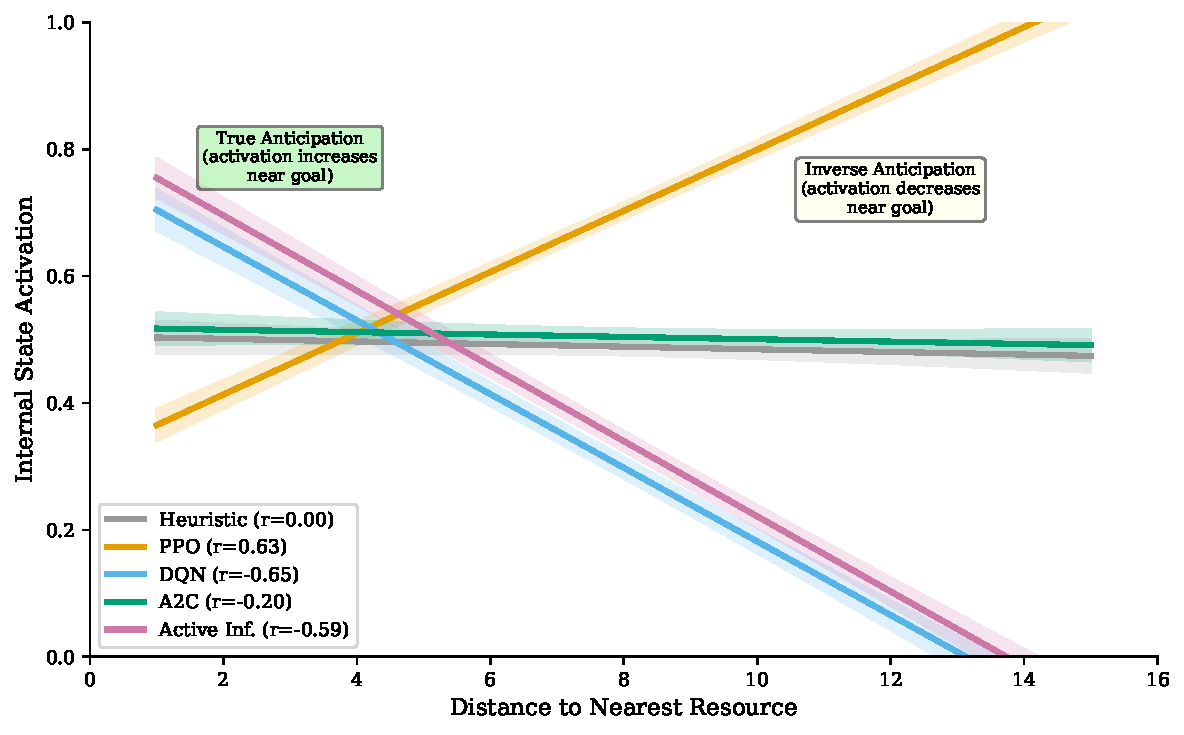
\includegraphics[width=0.95\linewidth]{figures/figure2_activation_distance.pdf}
    \caption{Internal state activation as a function of distance to nearest resource. DQN and Active Inference show true anticipation (negative slope)---activation increases as goals approach. PPO shows inverse anticipation (positive slope)---activation encodes uncertainty about distant goals. Shaded regions indicate 95\% confidence intervals.}
    \label{fig:activation_distance}
\end{figure}

\subsubsection{State-Dependent Valuation}

Unexpectedly, \textbf{A2C shows the highest SDV} (0.73), meaning its resource-seeking behavior is most strongly modulated by energy level. Active Inference shows moderate SDV (0.40), while other agents show zero (insufficient energy variation during testing).

\subsubsection{Frustration Intensification}

A2C (0.88) and PPO (0.69) show the strongest frustration responses after path blockage. DQN and Active Inference show minimal frustration intensification.

\subsubsection{Opportunity Cost Sensitivity}

Heuristic (1.0) and Active Inference (0.91) show high OCS, accurately weighing alternatives. RL agents show lower OCS, with PPO and DQN at zero.

\subsubsection{Extinction Resistance}

All agents show high ER (0.93--0.97), with no significant differentiation.

\subsection{Desire Profile Clustering}

\begin{figure}[t]
    \centering
    \begin{subfigure}[b]{0.48\textwidth}
        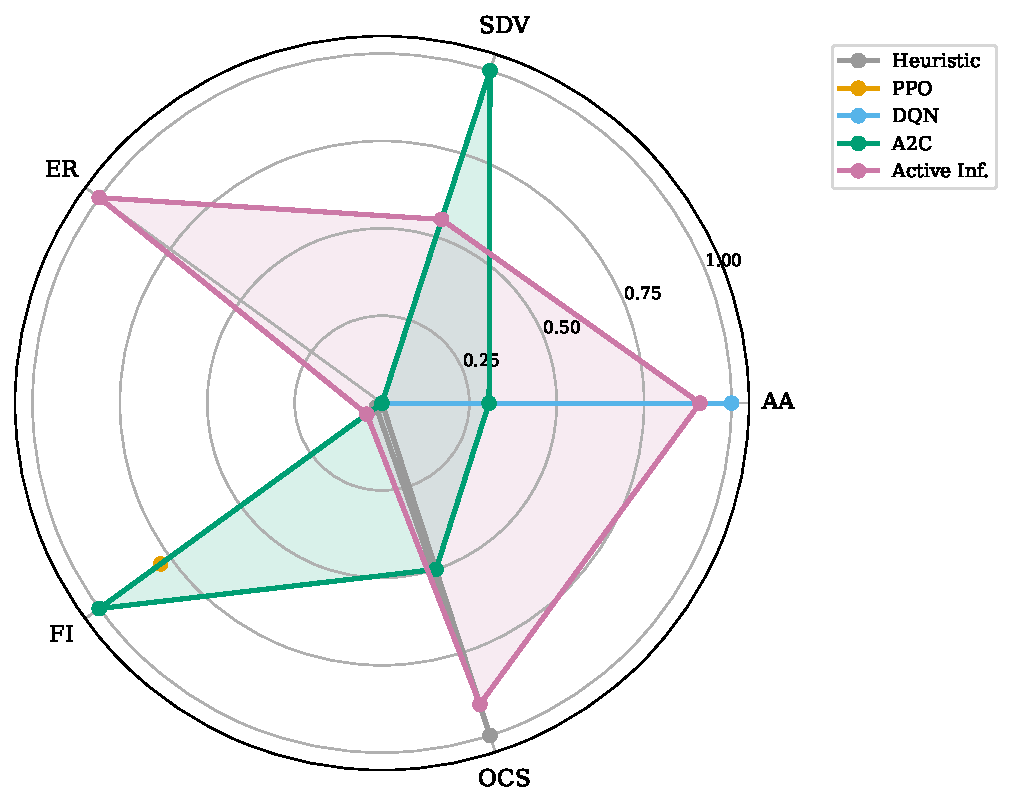
\includegraphics[width=\textwidth]{figures/figure1_radar.pdf}
        \caption{Radar chart of normalized desire profiles}
        \label{fig:radar}
    \end{subfigure}
    \hfill
    \begin{subfigure}[b]{0.48\textwidth}
        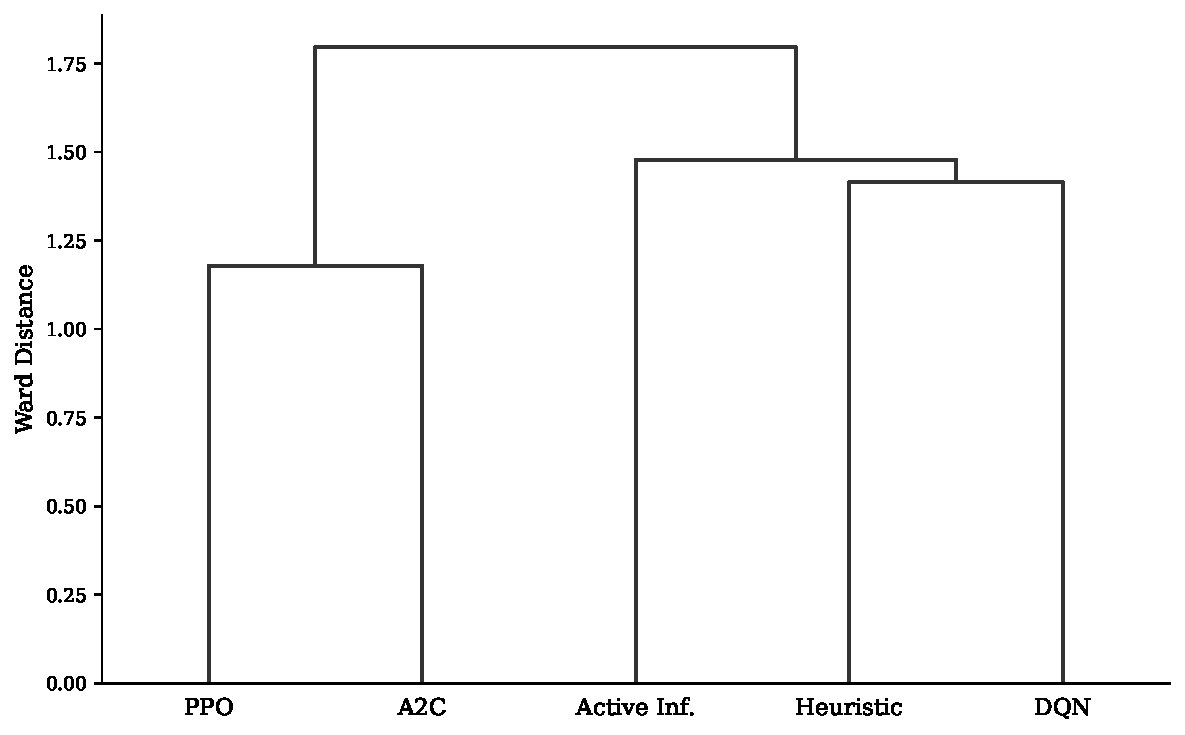
\includegraphics[width=\textwidth]{figures/figure3_clustering.pdf}
        \caption{Hierarchical clustering dendrogram}
        \label{fig:clustering}
    \end{subfigure}
    \caption{Multi-metric analysis of desire profiles. (a) Each agent exhibits a distinct pattern across five metrics. (b) Ward clustering reveals that agents do not cluster by framework (RL vs.\ Active Inference) but by architectural properties.}
    \label{fig:profiles}
\end{figure}

Figure~\ref{fig:profiles} shows the multi-dimensional desire profiles. Hierarchical clustering reveals that agents do not group by framework:
\begin{itemize}
    \item DQN and Active Inference cluster together (value-based prospective encoding)
    \item A2C clusters separately (high SDV and FI)
    \item PPO is an outlier (inverse anticipation)
    \item Heuristic clusters with Active Inference on OCS
\end{itemize}

\section{Discussion}

\subsection{Summary of Findings}

Our results challenge the hypothesis that Active Inference uniquely produces desire-like behavior. Instead:
\begin{enumerate}
    \item Both DQN and Active Inference show true anticipatory activation
    \item PPO shows \textit{inverse} anticipation, encoding uncertainty about distant goals
    \item A2C shows the highest state-dependent valuation and frustration response
    \item No single agent wins on all metrics
\end{enumerate}

\subsection{Why Value-Based Methods Show Anticipation}

DQN and Active Inference share a key architectural feature: explicit representation of expected future value. DQN's Q-function estimates cumulative future reward from each state-action pair; Active Inference's expected free energy explicitly computes anticipated outcomes. Both create prospective representations that may drive anticipatory internal dynamics.

In contrast, PPO's policy gradient optimizes action probabilities directly without explicitly representing future values in the feature space. The positive correlation we observe may reflect uncertainty encoding: distant goals are harder to reach, creating larger policy entropy and higher activation.

\subsection{The A2C Anomaly}

A2C's high SDV and FI scores suggest it develops representations that are more responsive to internal state (energy) and environmental perturbations (path blockage). This may reflect its architecture: the critic provides a baseline that tracks state value, while the actor adjusts behavior in response. The synchronous updates may create more reactive dynamics than PPO's clipped updates.

\subsection{Implications}

\paragraph{For AI alignment.} Our findings suggest that ``desire-likeness'' cannot be assessed by a single behavioral test. Agents may exhibit prospective representations (like anticipatory activation) without being globally goal-directed, or may show strong internal-state sensitivity without anticipation. Alignment research should consider the full profile of goal-directed behaviors.

\paragraph{For cognitive science.} The multi-dimensional nature of desire-like behavior in artificial agents parallels psychological findings that motivation has multiple components (wanting, liking, anticipating) that can dissociate \cite{berridge2009dissecting}.

\paragraph{For Active Inference.} Our results neither confirm nor refute Active Inference's special status. The framework produces anticipatory behavior, but so does value-based RL. The distinguishing feature may not be anticipation per se, but rather the integration of epistemic and pragmatic value---which we did not directly measure.

\subsection{Limitations}

\paragraph{Toy environment.} Our grid-world is far simpler than real-world environments. Results may not generalize to complex tasks.

\paragraph{Internal state operationalization.} We access different representations for different agents (hidden layers vs.\ belief states). A more unified measure would strengthen comparisons.

\paragraph{Limited training.} Agents may not have converged to optimal policies. Extended training might change the pattern.

\paragraph{Measurement artifacts.} The SDV zero scores for some agents may reflect measurement issues (insufficient energy variation) rather than absence of state-dependent valuation.

\subsection{Future Work}

\begin{enumerate}
    \item Test model-based RL agents (e.g., Dreamer, MuZero) to see if explicit planning produces anticipation
    \item Examine attention mechanisms in transformer-based agents
    \item Apply to larger-scale models (language models, vision models) to test scalability
    \item Develop predicates that directly measure epistemic vs.\ pragmatic value integration
\end{enumerate}

\section{Conclusion}

We investigated whether Active Inference agents exhibit unique behavioral signatures of ``desire-likeness.'' Testing five agent types across six predicates, we found that desire-likeness is multi-dimensional: no single framework dominates. Value-based methods (DQN, Active Inference) show true anticipatory activation; actor-critic methods (A2C) show high state-dependent valuation and frustration; PPO shows inverse anticipation. These results suggest that the \textit{architecture} of learning systems---not just the framework---determines which aspects of goal-directed behavior emerge. Future work should embrace multi-metric profiles rather than seeking single dissociating predicates.

\bibliographystyle{plain}
\begin{thebibliography}{10}

\bibitem{berridge2009dissecting}
K.~C. Berridge and M.~L. Kringelbach.
\newblock Affective neuroscience of pleasure: reward in humans and animals.
\newblock {\em Psychopharmacology}, 199(3):457--480, 2009.

\bibitem{bratman1987intention}
M.~Bratman.
\newblock {\em Intention, Plans, and Practical Reason}.
\newblock Harvard University Press, 1987.

\bibitem{dennett1987intentional}
D.~C. Dennett.
\newblock {\em The Intentional Stance}.
\newblock MIT Press, 1987.

\bibitem{dickinson1985actions}
A.~Dickinson.
\newblock Actions and habits: the development of behavioural autonomy.
\newblock {\em Philosophical Transactions of the Royal Society B}, 308(1135):67--78, 1985.

\bibitem{friston2010free}
K.~Friston.
\newblock The free-energy principle: a unified brain theory?
\newblock {\em Nature Reviews Neuroscience}, 11(2):127--138, 2010.

\bibitem{heins2022pymdp}
C.~Heins, B.~Millidge, et~al.
\newblock pymdp: A Python library for active inference in discrete state spaces.
\newblock {\em Journal of Open Source Software}, 7(73):4098, 2022.

\bibitem{lanillos2021active}
P.~Lanillos, C.~Meo, et~al.
\newblock Active inference in robotics and artificial agents: Survey and challenges.
\newblock {\em arXiv preprint arXiv:2112.01871}, 2021.

\bibitem{langdon2022model}
A.~J. Langdon, M.~J. Sharpe, et~al.
\newblock Model-based and model-free decision making in artificial agents.
\newblock {\em Current Opinion in Behavioral Sciences}, 44:101103, 2022.

\bibitem{millidge2020relationship}
B.~Millidge, A.~Tschantz, and C.~L. Buckley.
\newblock Whence the expected free energy?
\newblock {\em Neural Computation}, 33(2):447--482, 2021.

\bibitem{parr2022active}
T.~Parr, G.~Pezzulo, and K.~J. Friston.
\newblock {\em Active Inference: The Free Energy Principle in Mind, Brain, and Behavior}.
\newblock MIT Press, 2022.

\bibitem{raffin2021stable}
A.~Raffin, A.~Hill, et~al.
\newblock Stable-Baselines3: Reliable reinforcement learning implementations.
\newblock {\em Journal of Machine Learning Research}, 22(268):1--8, 2021.

\bibitem{schulman2017proximal}
J.~Schulman, F.~Wolski, et~al.
\newblock Proximal policy optimization algorithms.
\newblock {\em arXiv preprint arXiv:1707.06347}, 2017.

\bibitem{seth2021being}
A.~K. Seth.
\newblock {\em Being You: A New Science of Consciousness}.
\newblock Dutton, 2021.

\bibitem{smith2022step}
R.~Smith, K.~J. Friston, and C.~J. Whyte.
\newblock A step-by-step tutorial on active inference and its application to empirical data.
\newblock {\em Journal of Mathematical Psychology}, 107:102632, 2022.

\bibitem{tschantz2020reinforcement}
A.~Tschantz, B.~Millidge, et~al.
\newblock Reinforcement learning through active inference.
\newblock {\em arXiv preprint arXiv:2002.12636}, 2020.

\end{thebibliography}

\newpage
\appendix
\section{Supplementary Material}

\subsection{Environment Details}

The foraging environment is implemented using the Gymnasium API. The observation space consists of:
\begin{itemize}
    \item Local view: $(11, 11, 3)$ tensor with channels for terrain, resources, and agent position
    \item Energy: Scalar normalized to $[0, 1]$
    \item Position: $(x, y)$ normalized to $[0, 1]$
    \item Step: Normalized timestep
\end{itemize}

Action space: \{UP, DOWN, LEFT, RIGHT, STAY, CONSUME\}

\subsection{Active Inference Implementation Details}

The Active Inference agent uses a factorized state space:
\begin{itemize}
    \item Factor 1: Discretized position (400 states for $20 \times 20$ grid)
    \item Factor 2: Discretized energy level (10 bins)
\end{itemize}

The A matrix (observation model) includes noise ($\sim$15\% observation error) to prevent belief collapse. The B matrix (transition model) encodes deterministic dynamics with small stochasticity. The C matrix (preferences) encodes high preference for high-energy states.

Expected free energy is computed using:
\begin{equation}
    G(\pi) = \sum_\tau \mathbb{E}_{Q(o_\tau, s_\tau | \pi)} \left[ \log Q(s_\tau | \pi) - \log P(o_\tau, s_\tau) \right]
\end{equation}

We use beam search (width 20) to evaluate policies, selecting actions with lowest $G$.

\subsection{Full Statistical Results}

\paragraph{Anticipatory Activation (DQN vs.\ Active Inference).}
\begin{itemize}
    \item DQN: $r = -0.652$ (true anticipation)
    \item Active Inference: $r = -0.593$ (true anticipation)
    \item Mann-Whitney $U = 0.0$, $p < 0.001$
    \item Cohen's $d = 8.22$ (large effect)
    \item Bootstrap 95\% CI for difference: $[0.114, 0.141]$
\end{itemize}

\paragraph{Kruskal-Wallis omnibus tests.}
\begin{itemize}
    \item AA: $H = 48.60$, $p < 0.001$
    \item OCS: $H = 47.57$, $p < 0.001$
    \item SDV: $H = 48.50$, $p < 0.001$
\end{itemize}

\subsection{Raw Data Availability}

Raw trial-level data and code are available at: \url{https://github.com/paulfryer/desire}

\end{document}
